\documentclass[12pt]{amsart}
\usepackage{preamble}
%\DeclareRobustCommand{\flippedSlash}{\text{\reflectbox{$\setminus$}}}

\begin{document}
\begin{center}
   \textsc{Math 676 Computational Group Theory. HW 5\\ Ian Jorquera}
\end{center}
\vspace{1em}

\begin{itemize}
   \item[(22)]
   \begin{enumerate}[label= (\alph*)]
    \item To find the presentation for the generators $(1,2,3)$ and $(2,3)$
     I used GAP with the following commands\\
    

   iso := IsomorphismFpGroupByGenerators(SymmetricGroup(3), [(1,2,3), (2,3)]);\\
   fp := Image( iso );\\
   RelatorsOfFpGroup( fp );\\

   which gave the following presentation $G=\ip{a,b|a^3,b^2,(a^{-1}b)^2}$. 
   To show that this is in fact $S_3$ we can first show 
   that the $a=(1,2,3)$ and $b=(2,3)$ satisfy the relations. 
   Notice $(1,2,3)^3=()$, and $(2,3)^2=()$ and $(2,3)^{-1}(1,2,3)(2,3)^{-1}(1,2,3)=()$. 
   This shows that the presentation at least contains $S_3$, as 
   there is a injective homomorphism into our presentation. 
   To show that the presentation is no bigger we can consider the order via a coset enumeration.
   Let $S=\ip{a}$ and so $|S|=3$ and we get the following coset enumeration

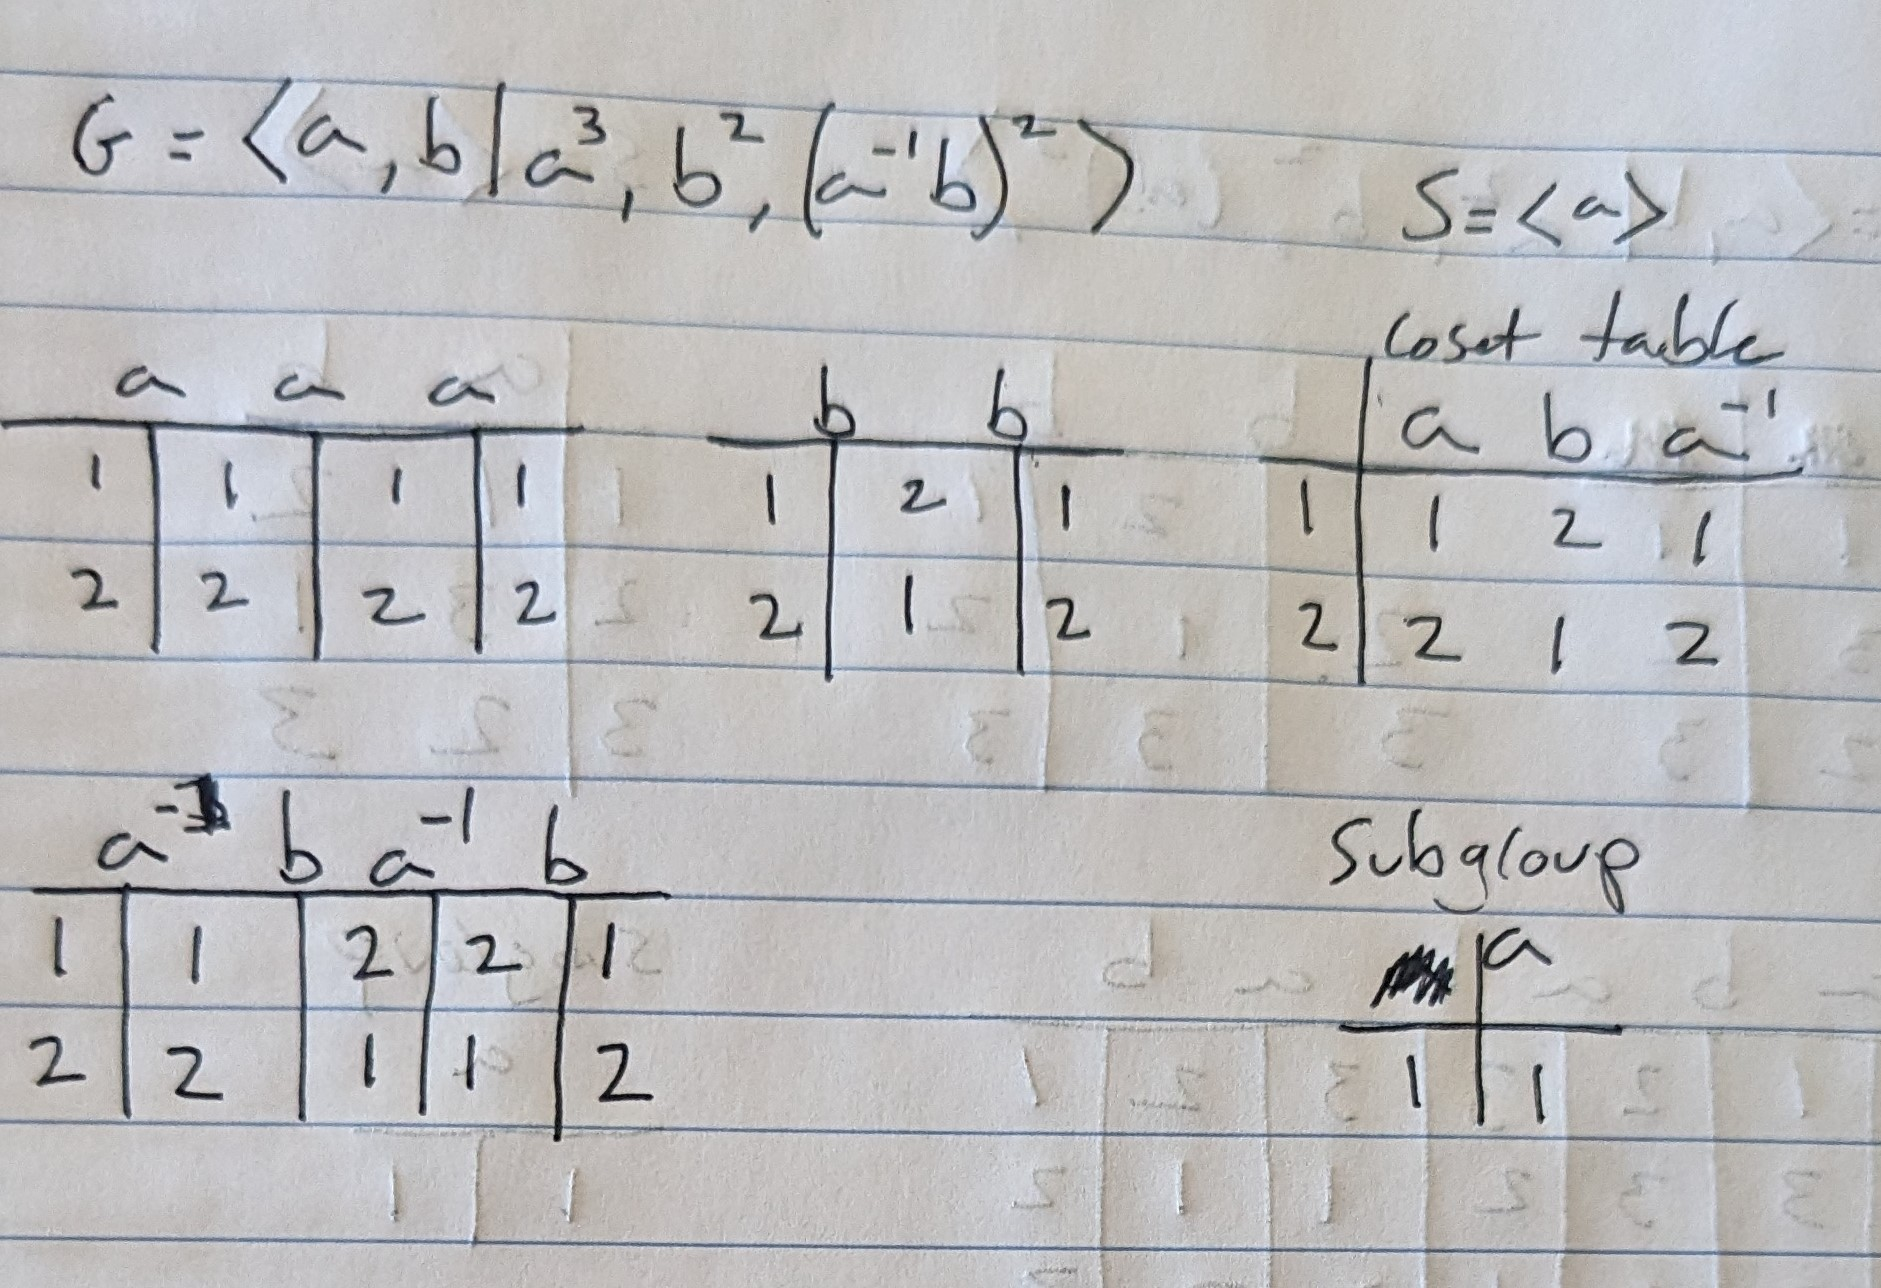
\includegraphics[scale=.15]{676parta.jpg}


   This shows that $|G/S|=2$ and so $|G|=6$, meaning $G\cong S_3$.

   \item To find the presentation I used GAP and found with the generators $(1,2,3), (2,3), (1,2)$
   were the presentation would be $G=\ip{a,b,c|a^3,b^2,c^2,bac}$. 
   To show that this is in fact $S_3$ we can first show 
   that the $a=(1,2,3)$, $b=(2,3)$, and $c=(1,2)$ satisfy these relations. % idk do this correctly
   Notice $(1,2,3)^3=()$, and $(2,3)^2=()$, and $(1,2)^2=()$ and $(2,3)(1,2,3)(1,2)=()$. 
   This shows that the presentation at least contains $S_3$, as 
   there this defines an injective homomorphism into our presentation. 
   To show that the presentation is no bigger we can consider the order via a coset enumeration.
   Let $S=\ip{a}$ and so $|S|=3$ and we get the following coset enumeration

   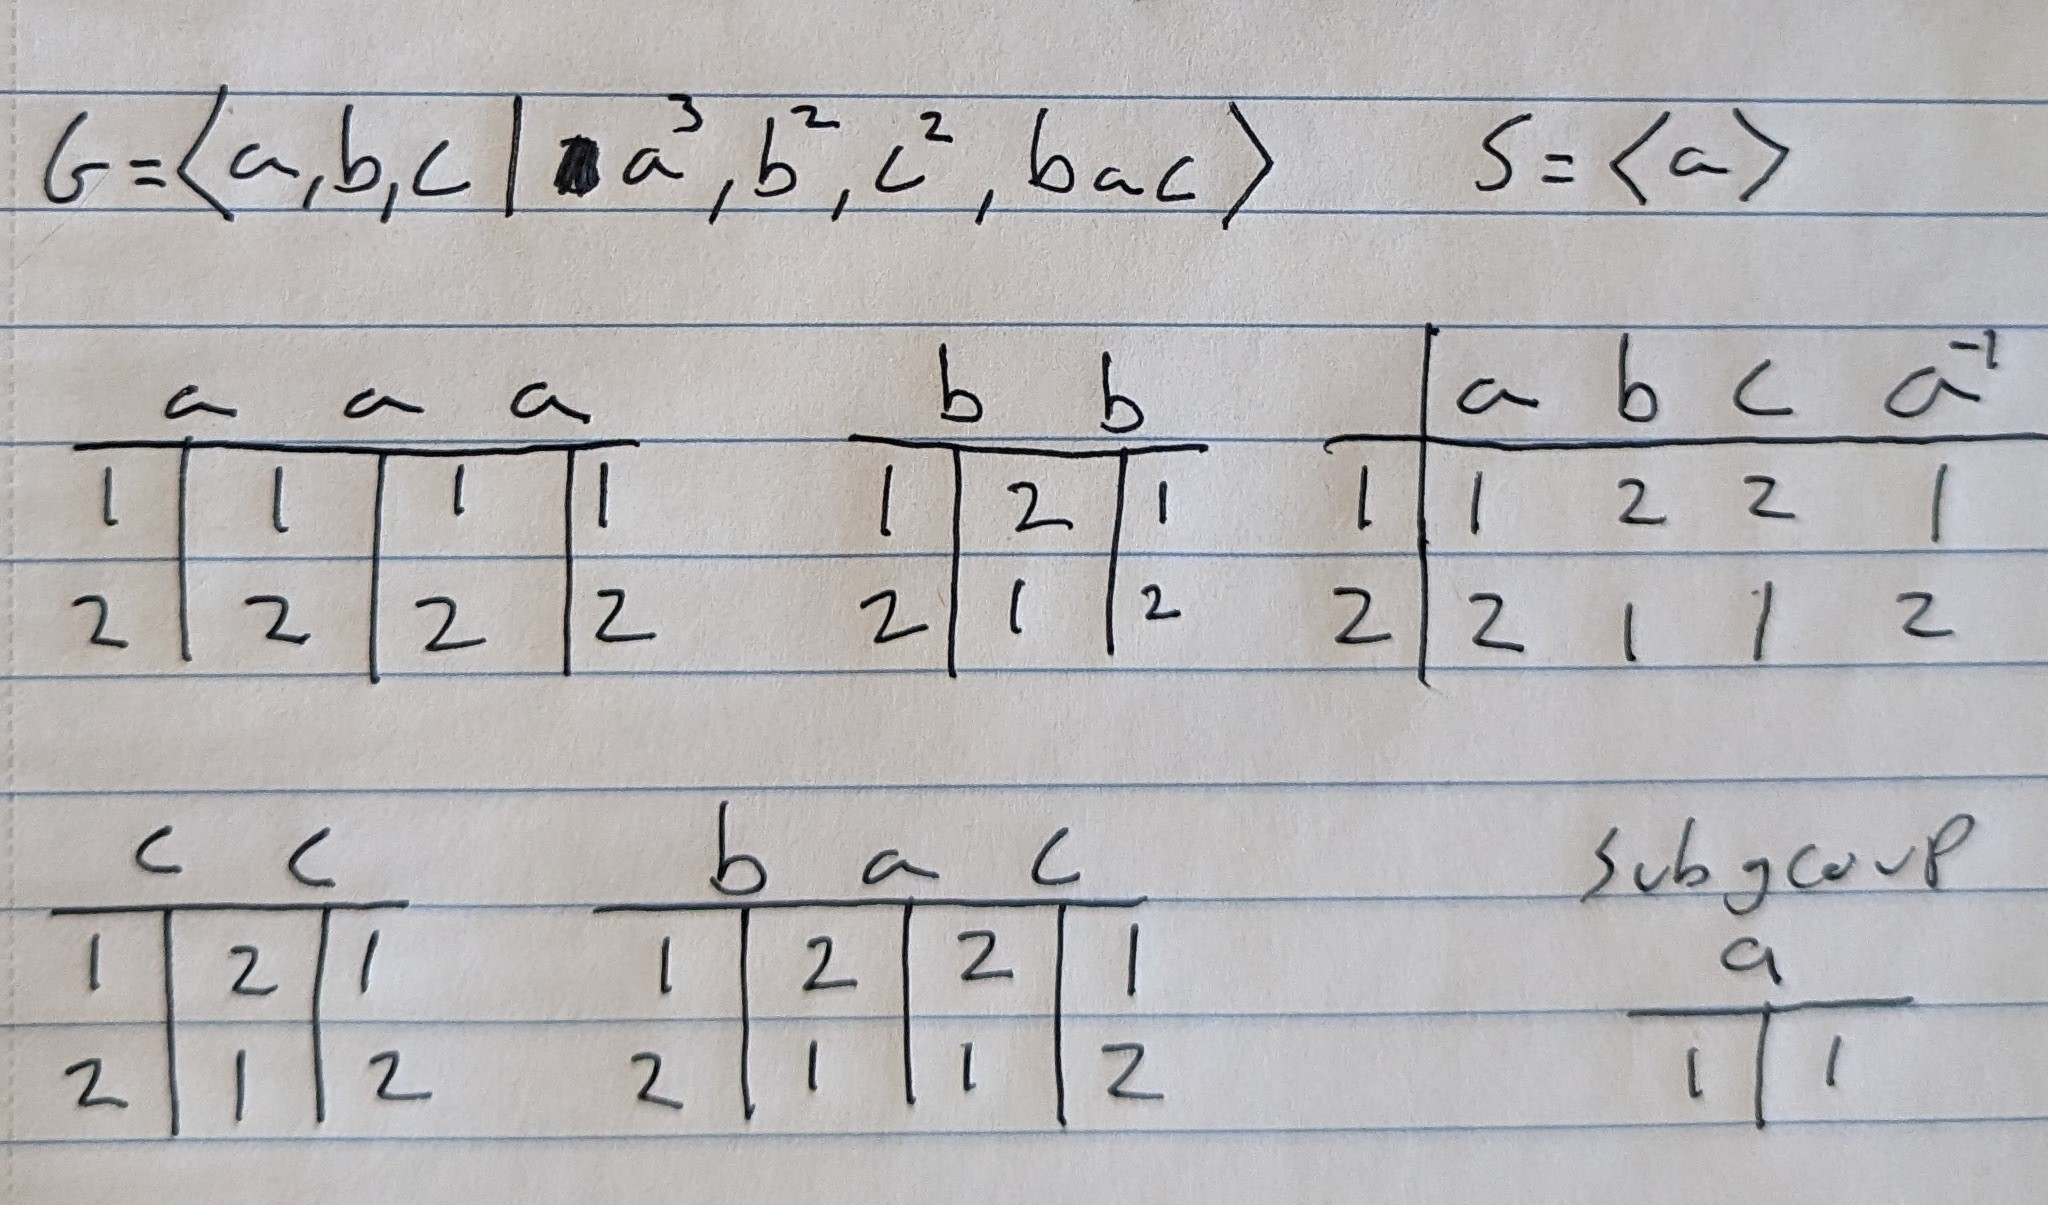
\includegraphics[scale=.15]{676partb.jpg}

   This shows that $|G/S|=2$ and so $|G|=6$, meaning $G\cong S_3$.

   \item To find the presentation I used GAP and found with the generators $(1,2), (2,3)$
   were the presentation would be $G=\ip{a,b|a^2,b^2,(ab)^3}$. 
   To show that this is in fact $S_3$ we can first show 
   that the $a=(1,2)$ and $a=(2,3)$ satisfy these relations. % idk do this correctly
   Notice $(1,2)^2=()$, and $(2,3)^2=()$ and $(1,2)(2,3)(1,2)(2,3)(1,2)(2,3)=()$. 
   This shows that the presentation at least contains $S_3$, as 
   there is an injective homomorphism into our presentation. 
   To show that the presentation is no bigger we can consider the order via a coset enumeration.
   Let $S=\ip{b}$ and so $|S|=2$ and we get the following coset enumeration

   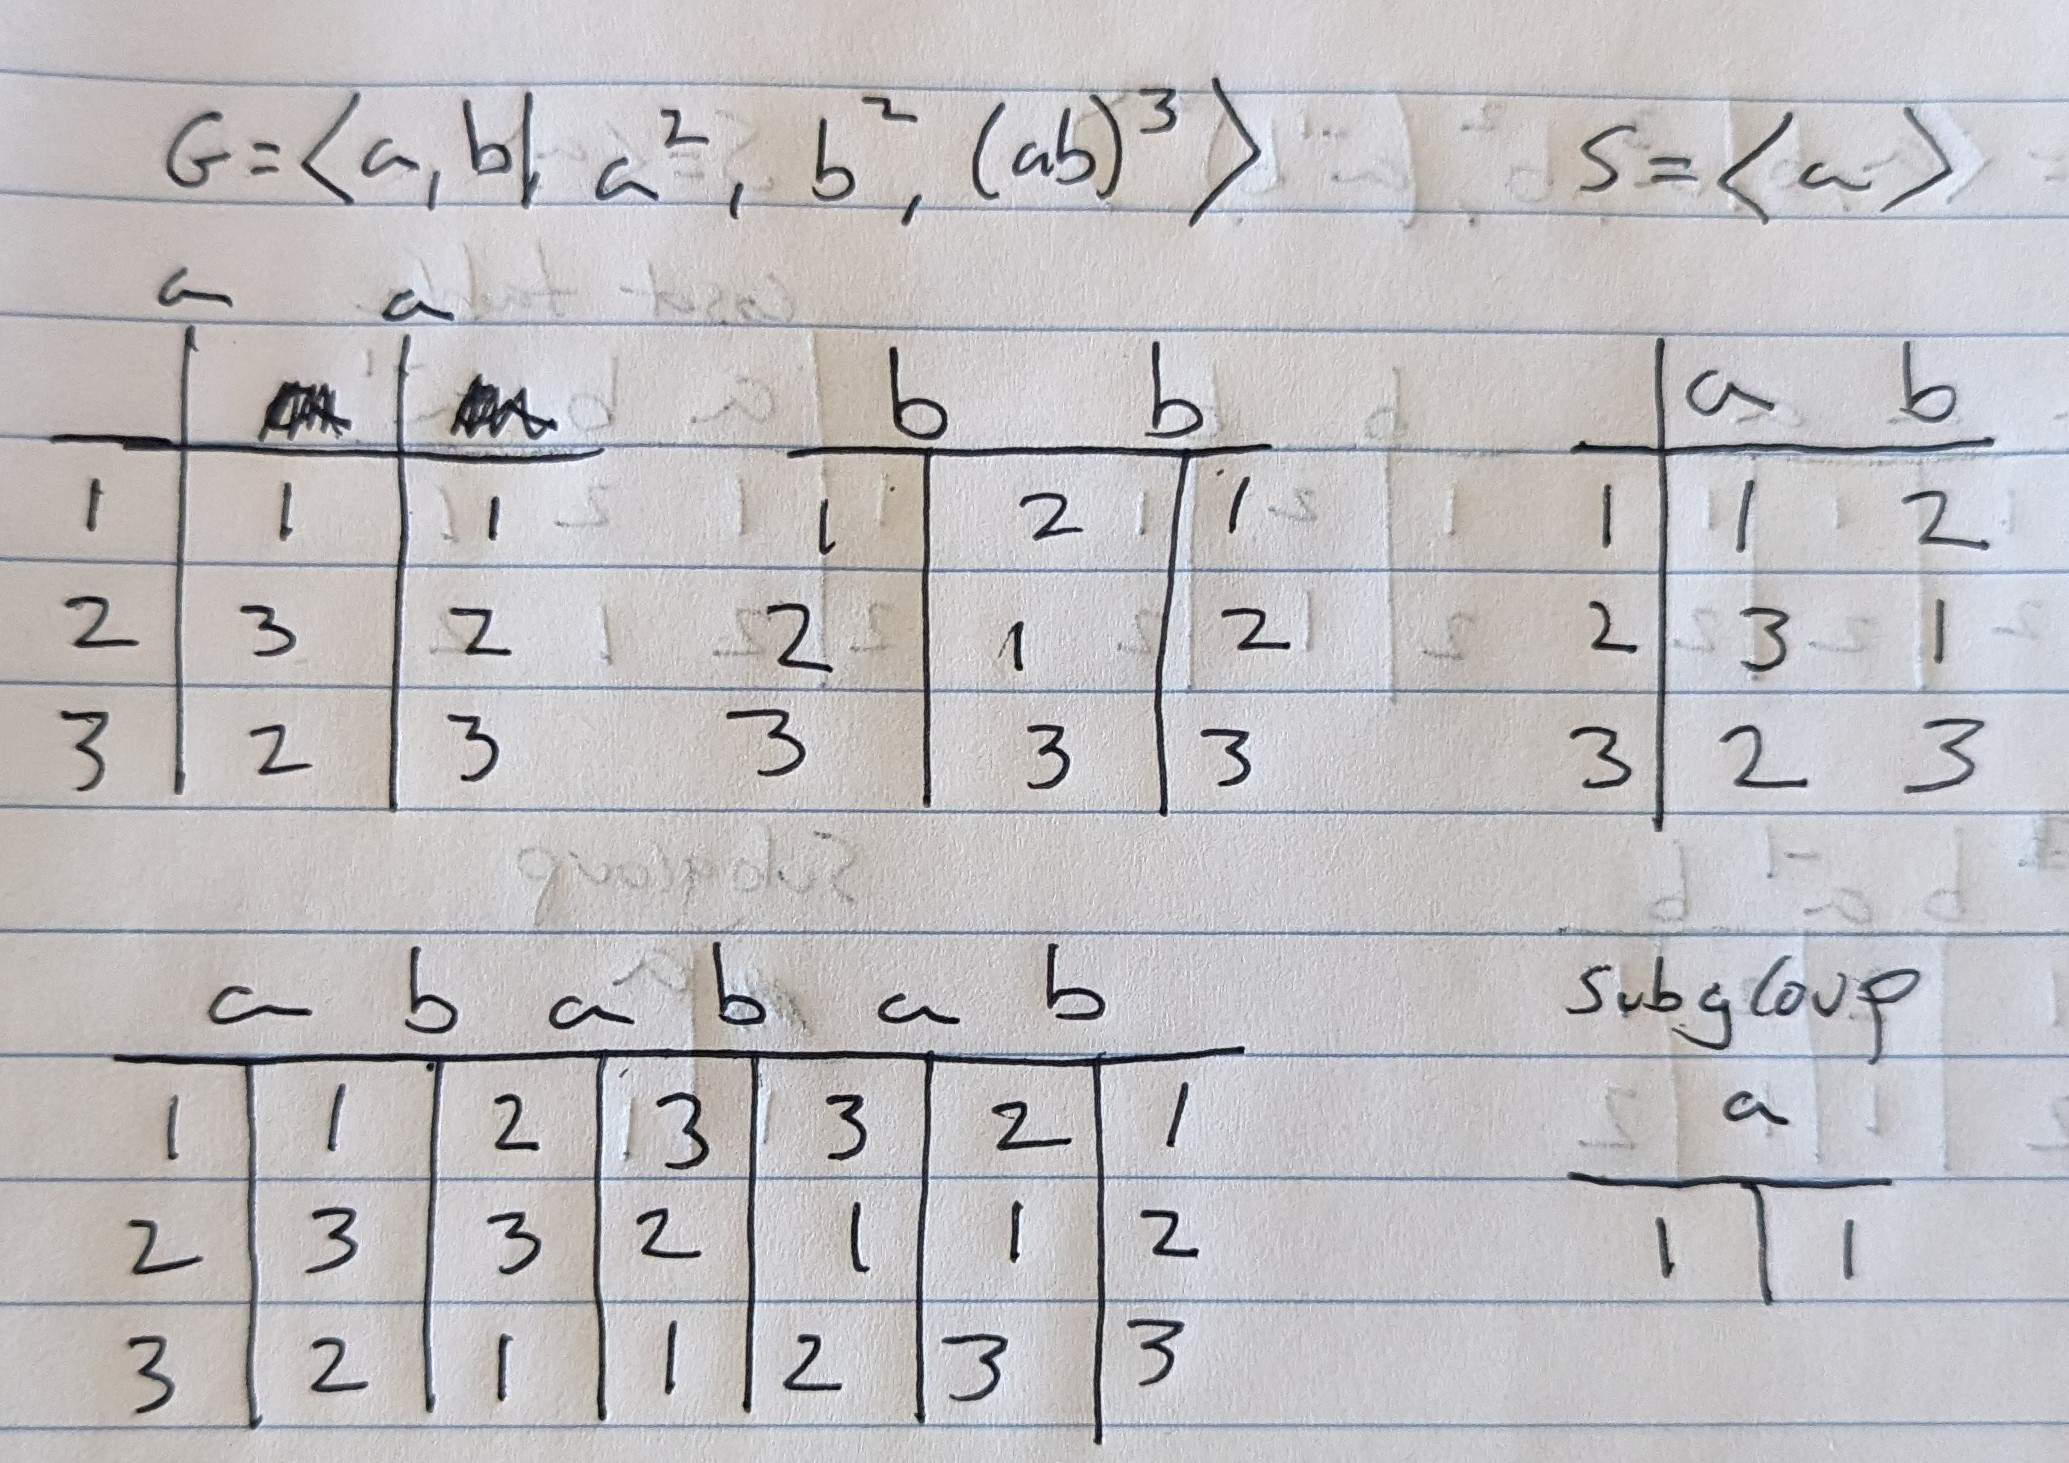
\includegraphics[scale=.15]{676partc.jpg}

   This show that $|G/S|=3$ and so $|G|=6$, meaning $G\cong S_3$.
   \item 
    Notice first that $C_2^2$ is a normal subgroup of $S_4$ which we can determine with GAP\\
    
    g:=SymmetricGroup(4);\\
    List( NormalSubgroups(g), StructureDescription );\\
    
    Which return S4, A4, C2 $\times$ C2, 1. We can also notice that $S_4/C_2^2\cong S_3$

      IsomorphismGroups(s4/Group([ (1,4)(2,3), (1,2)(3,4) ]),SymmetricGroup(3));\\


      To construct a presentation for $S_4$ we can use the fact that $S_4\cong C_2^2\rtimes S_3$
      and that $\underbar{n}={(1,4)(2,3), (1,2)(3,4)}$ is a generating set for $C_2^2$ 
      whose presentation is $\ip{x,y|x^2,y^2,(xy)^2}$. Then notice that we 
      have a generating set $S_4=\ip{C_2^2,(1,2,3), (2,3)}$ and 
      $S_4/C_2^2\cong \ip{a,b|a^3,b^2,(a^{-1}b)^2}$

      This means that we can construct a presentation to be the following 

      $G=\ip{a,b,x,y|x^2,y^2,(xy)^2,a^3,b^2,(a^{-1}b)^2,x^a=xy,x^b=x,y^a=x,y^b=xy}$


    %c22 := DirectProduct(CyclicGroup(2),CyclicGroup(2));
%<pc group of size 4 with 2 generators>
%gap> ac22:=AutomorphismGroup(c22);
%<group with 4 generators>
%gap> SemidirectProduct(ac22,IdentityMapping(ac22),c22);
%<pc group with 4 generators>
%gap> IsomorphismGroups(SemidirectProduct(ac22,IdentityMapping(ac22),c22),SymmetricGroup(4));
\end{enumerate}

\item[(25)] All my work is shown in the picture below. (a) Notice that in the 
coset enumeration $4$ cosets were found showing that $[G:S]=4$. 
(b) The below coset table is an augmented coset table which 
defines the Scheier generators as follows $a=a$, $c=bab^{-1}$, 
$d=b^{-1}ab$, $e=b^4$ and $f=b^2ab^{-2}$.

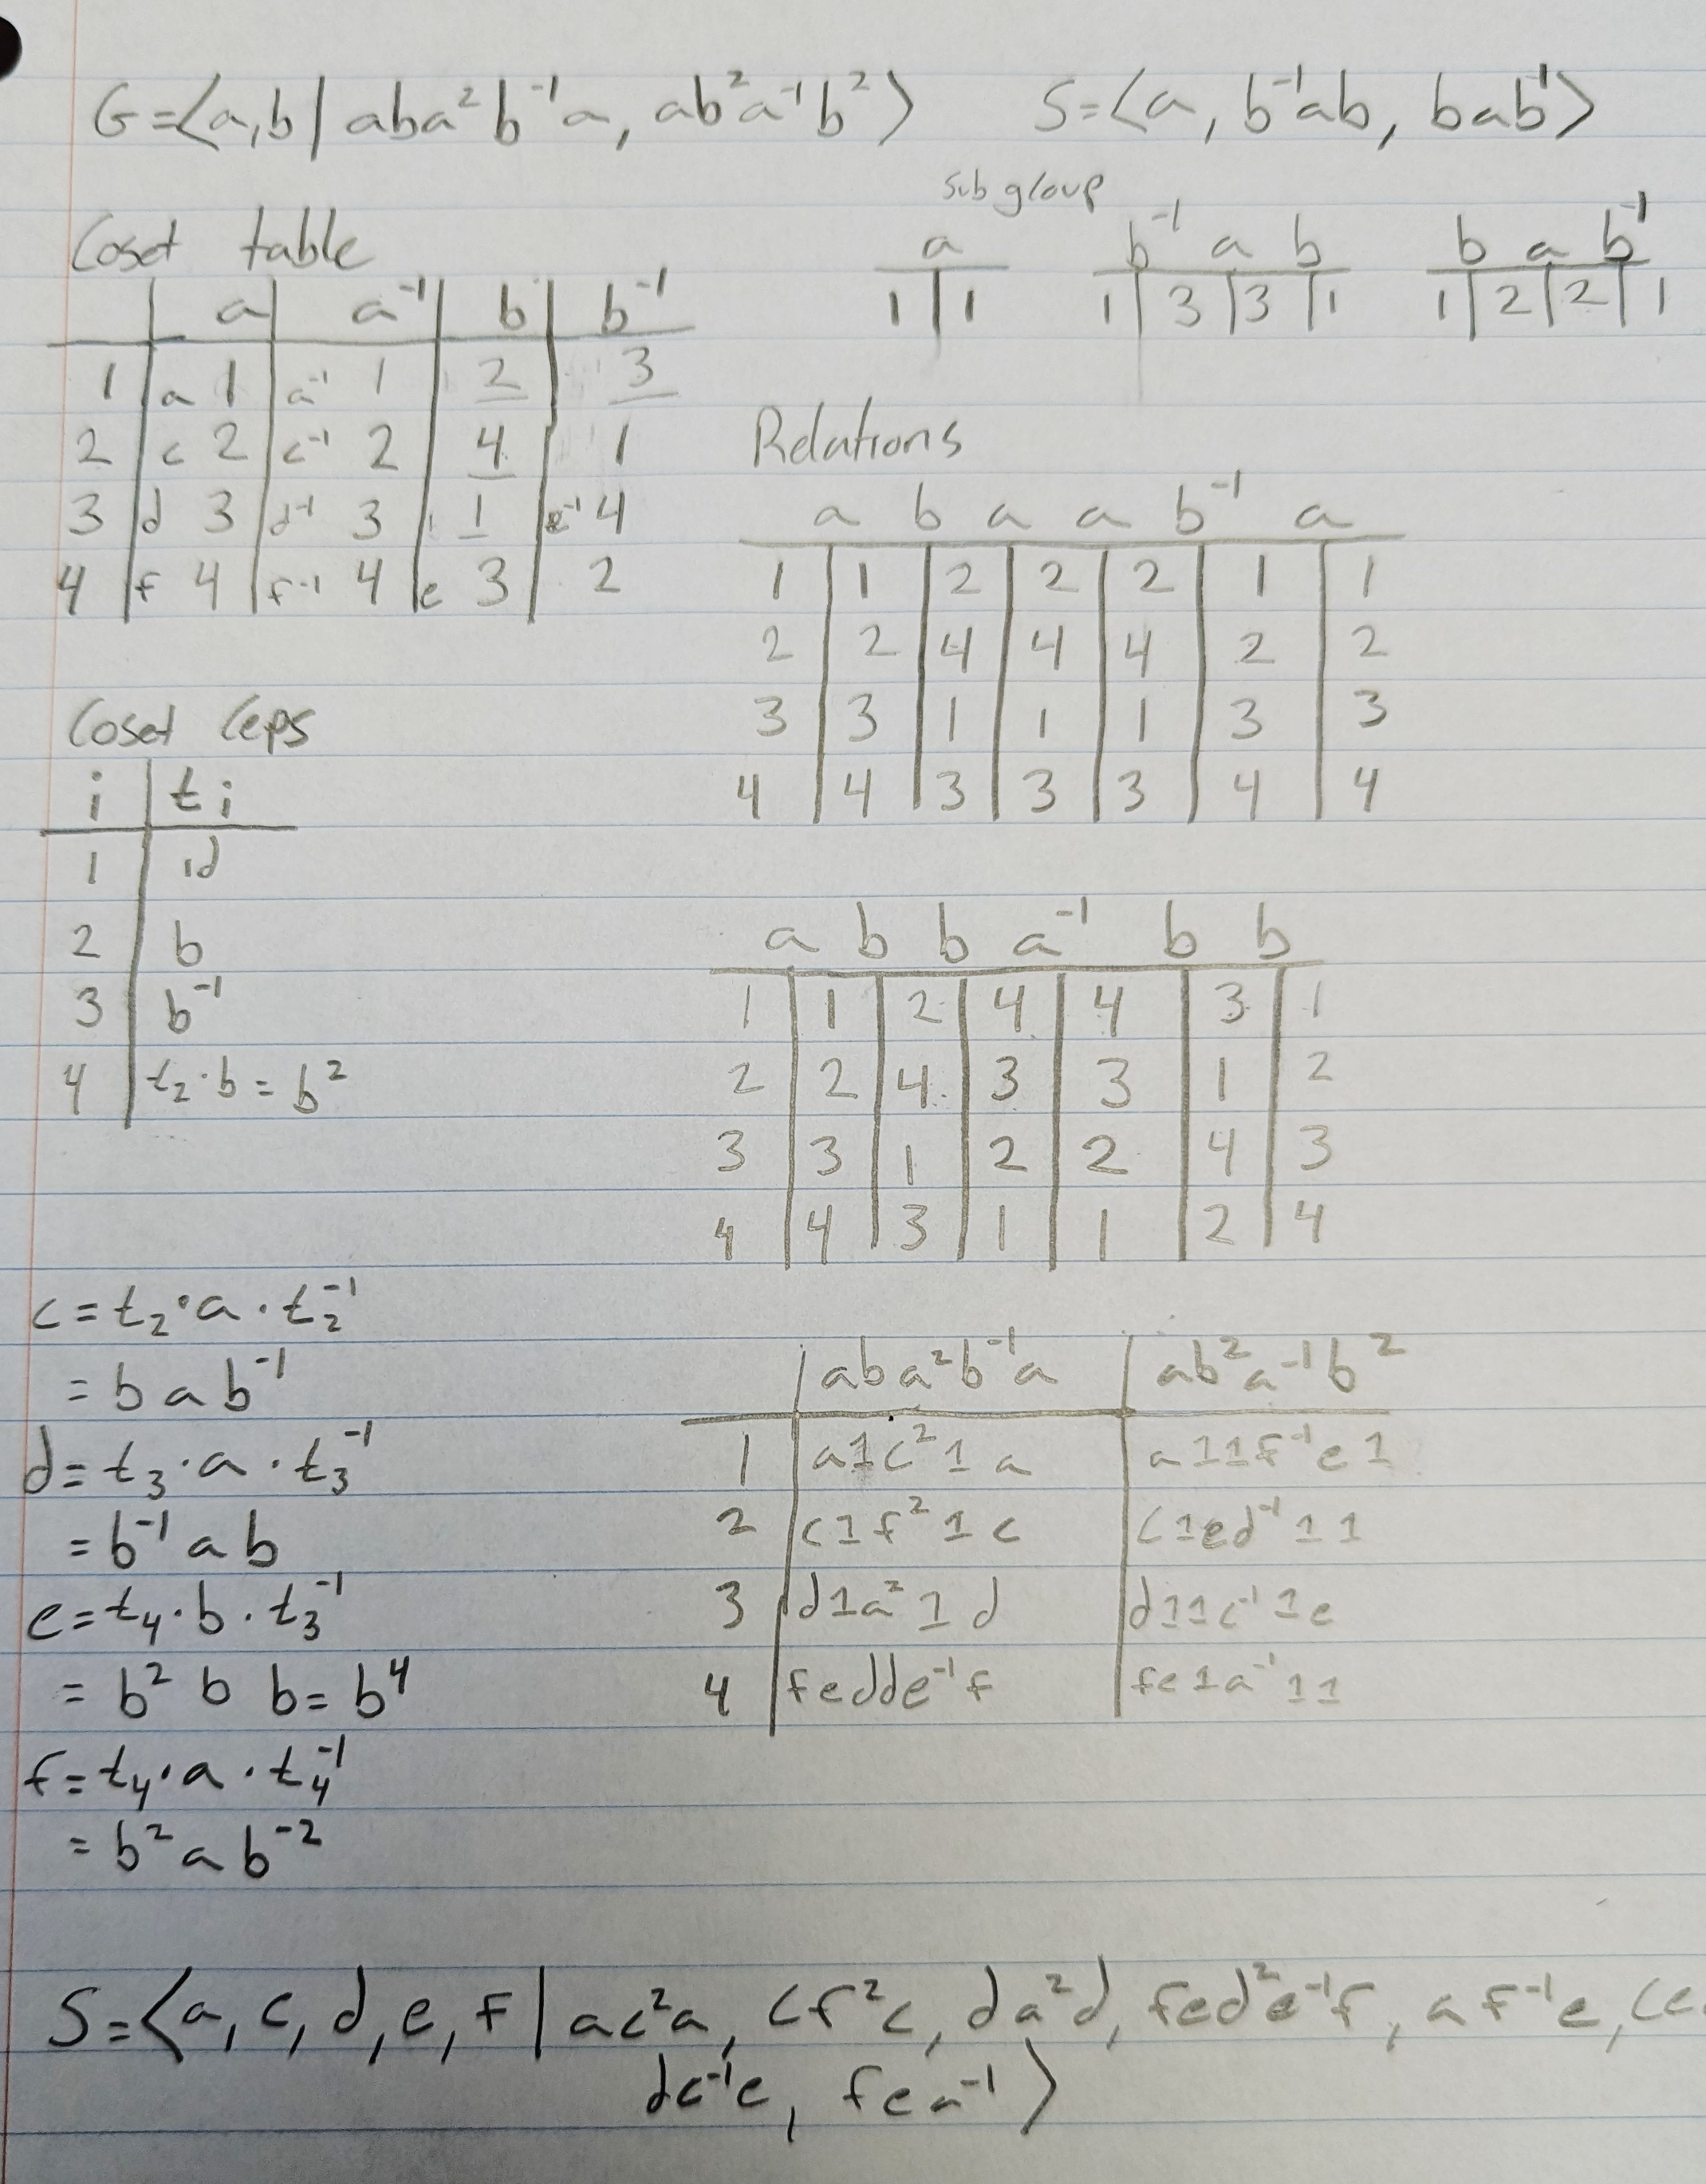
\includegraphics[scale=.2]{676hw425.jpg}

We also found that the presentation for $S$ is 

$S=\ip{a,c,d,e,f|ac^2a,cf^c,da^d,fed^2e^{-1}f,af^{-1}e,ced^{-1},dc^{-1}e,fea^{-1}}$

\end{itemize}


\end{document}